
\begin{document}

\chapter{Design}

\label{chapter:design}

\section{Agents}

% Single agent PDF

\begin{equation}
    P_a(x, y, t_0, t_m) = \int^{t_m}_{t_0}
    \mathcal{N}(\zeta_a(t), \alpha \cdot (t - t_0)^2 + \beta, x, y) \cdot
    (t_m - t)^{\gamma} \,\mathrm{d}t
    \label{eq:singleprob}
\end{equation}

Where $\mathcal{N}(\mu, \sigma^2, x, y)$ is the evaluation of a 3D normal
distribution centered at $(\mu_x, \mu_y)$ with a variance of $\sigma^2$ at $(x,
y)$.

% Multiple agent PDF

\begin{equation}
    P_A(x, y, t_0, t_m) = \frac{\mathlarger{\sum_{a \in A}
    P_a(x, y, t_0, t_m)}}{|A|}
    \label{eq:prob}
\end{equation}

% Obstacle equation

\begin{equation}
    \zeta_a(t) =
        \begin{cases}
            I_a + \mathlarger{\int_{T_a}^{t}} \dot{\zeta_a}(\lambda) \, \mathrm{d}\lambda
            & \text{if } t \geq T_a \\
            \tilde{\zeta_a}(t) & \text{if } t < T_a
        \end{cases}
    \label{eq:obs_pred}
\end{equation}

\begin{equation}
    \tilde{\zeta_a}(t) = I^{(0)}_a + \int_{0}^{t} \dot{\zeta_a}(\lambda)
    + \rho \, \mathrm{d}\lambda
    \label{eq:obs_observed}
\end{equation}

\begin{figure}[h!]

    \centering

    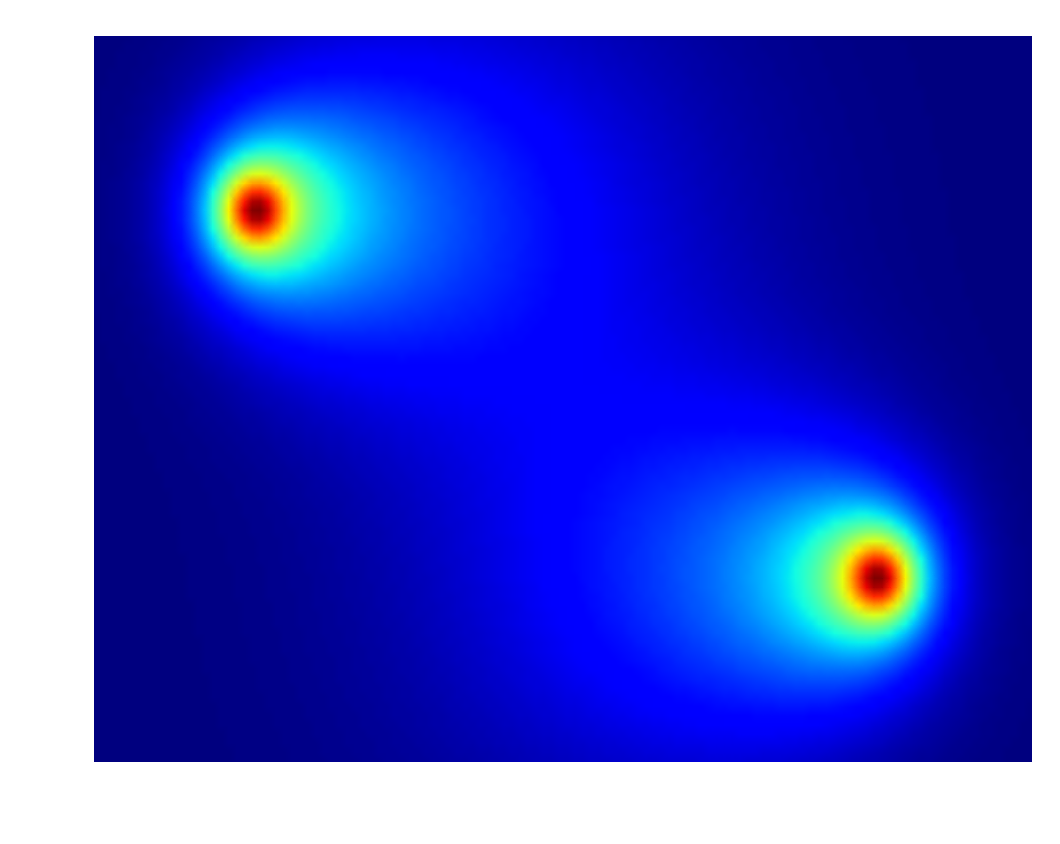
\includegraphics[width=0.24\linewidth]{figs/agent_1}
    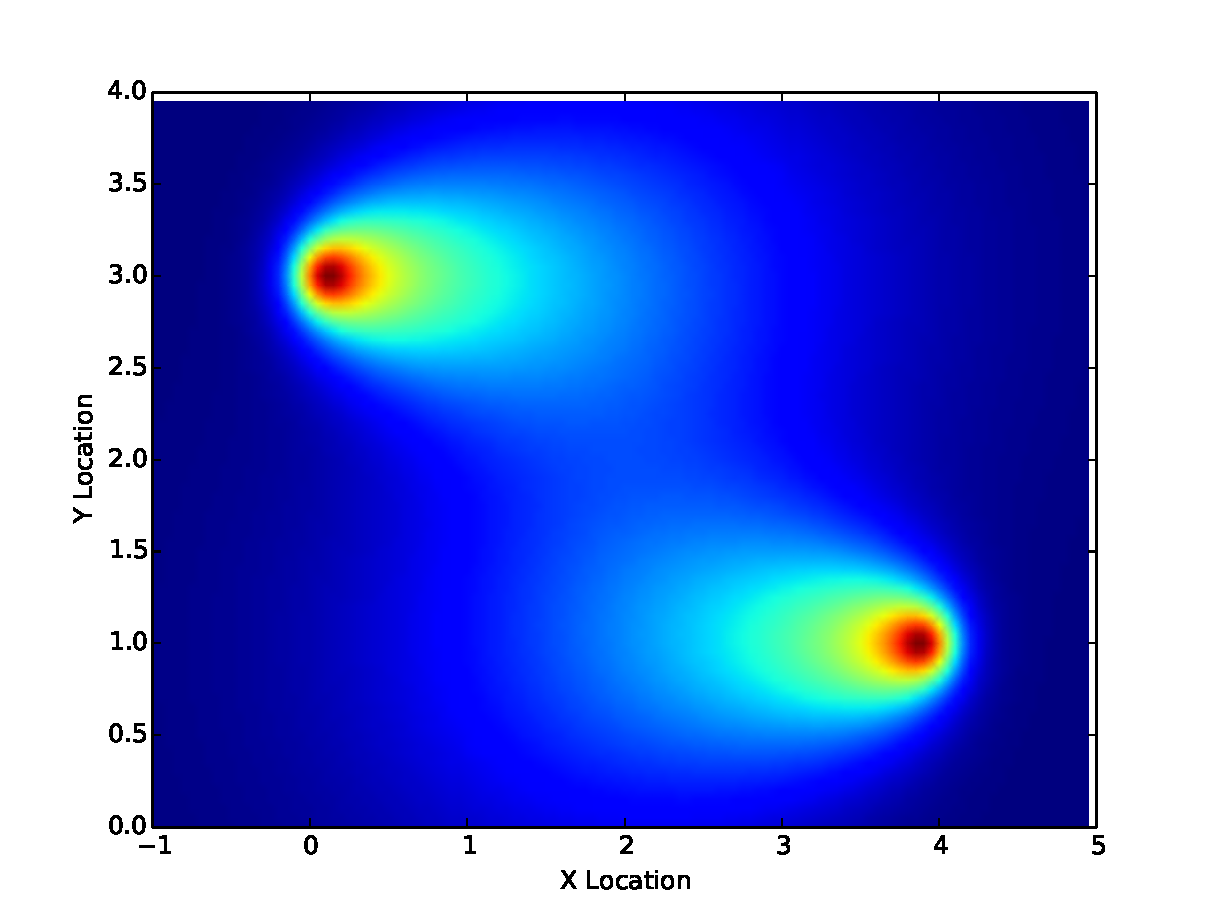
\includegraphics[width=0.24\linewidth]{figs/agent_2}
    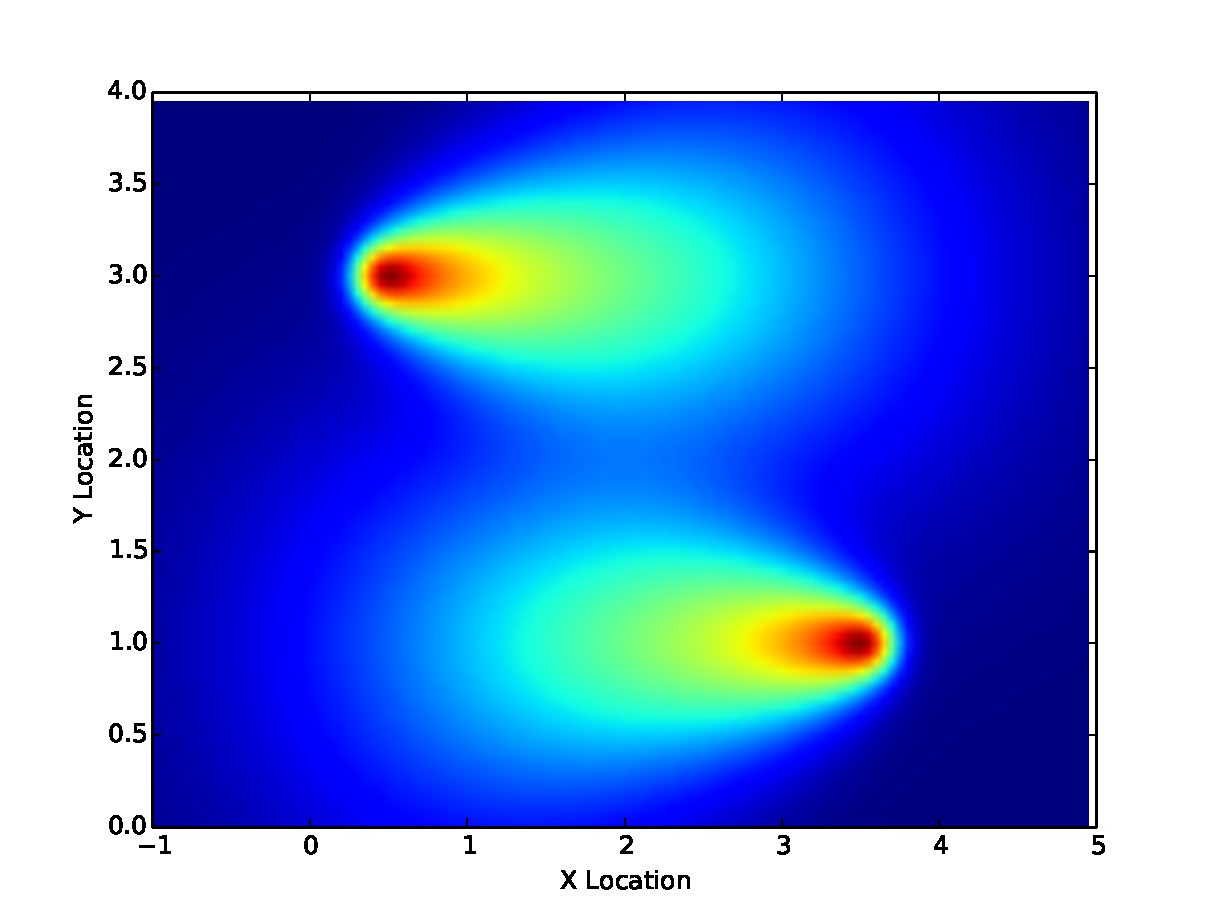
\includegraphics[width=0.24\linewidth]{figs/agent_3}
    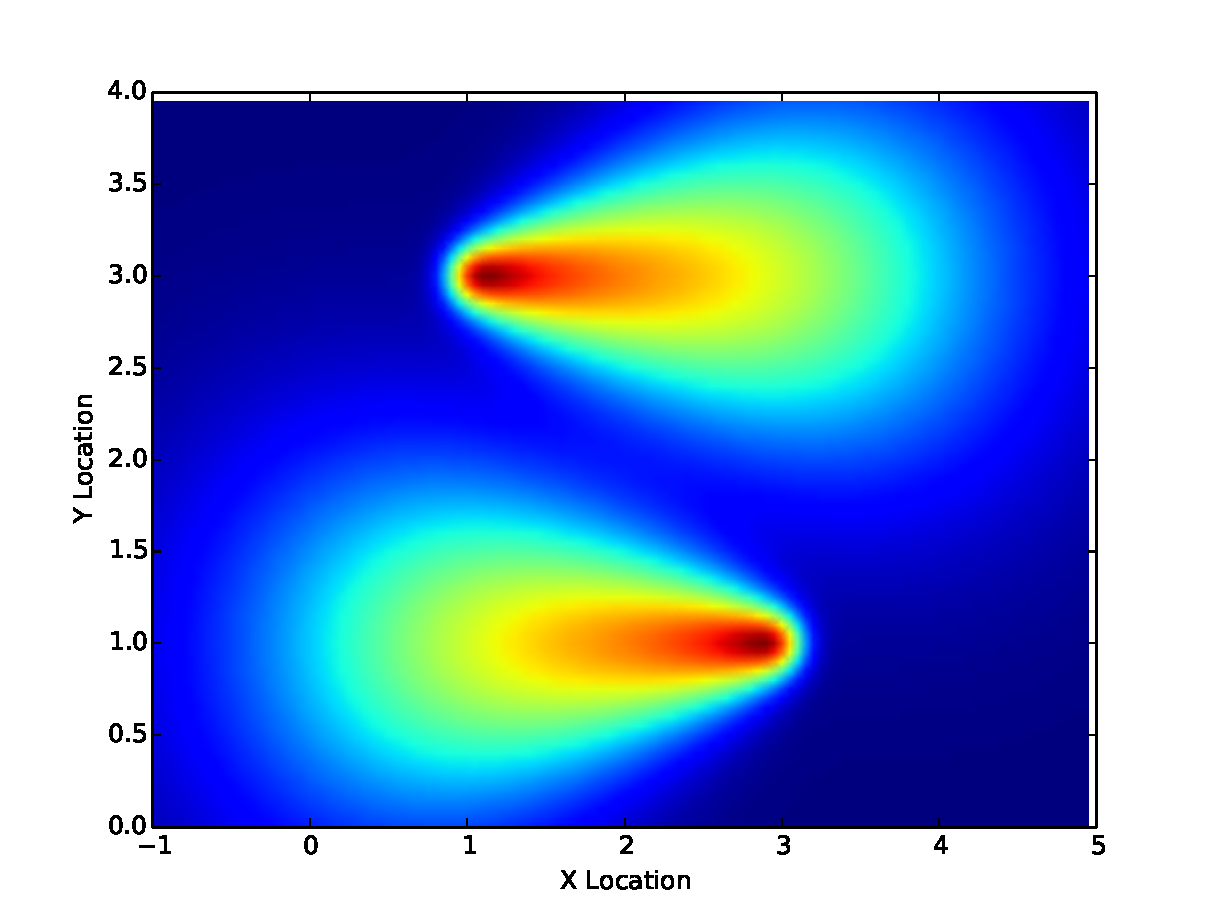
\includegraphics[width=0.24\linewidth]{figs/agent_4} \\
    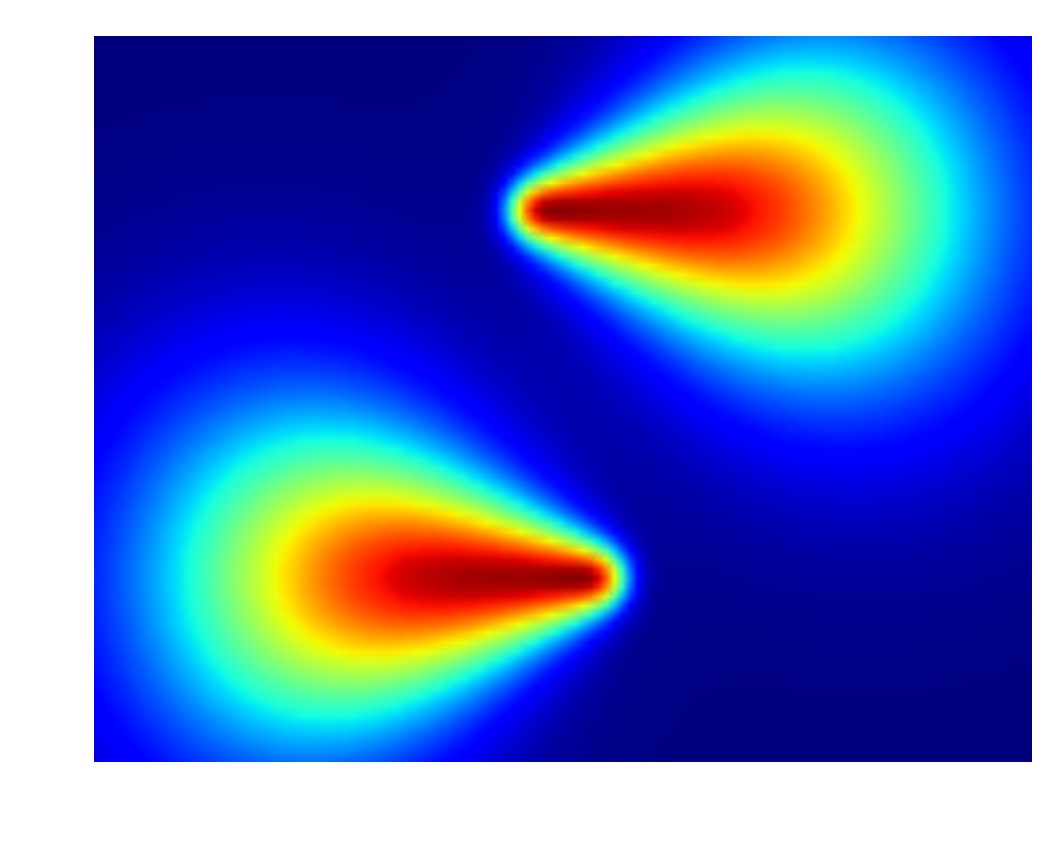
\includegraphics[width=0.24\linewidth]{figs/agent_5}
    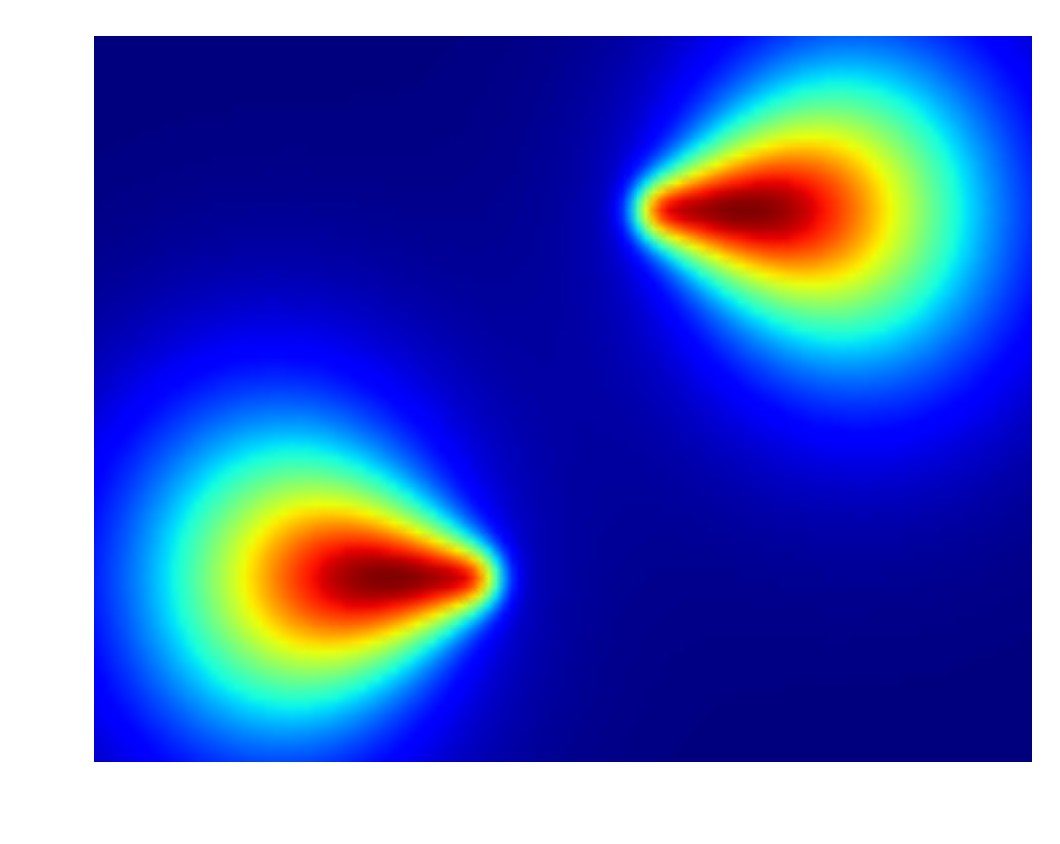
\includegraphics[width=0.24\linewidth]{figs/agent_6}
    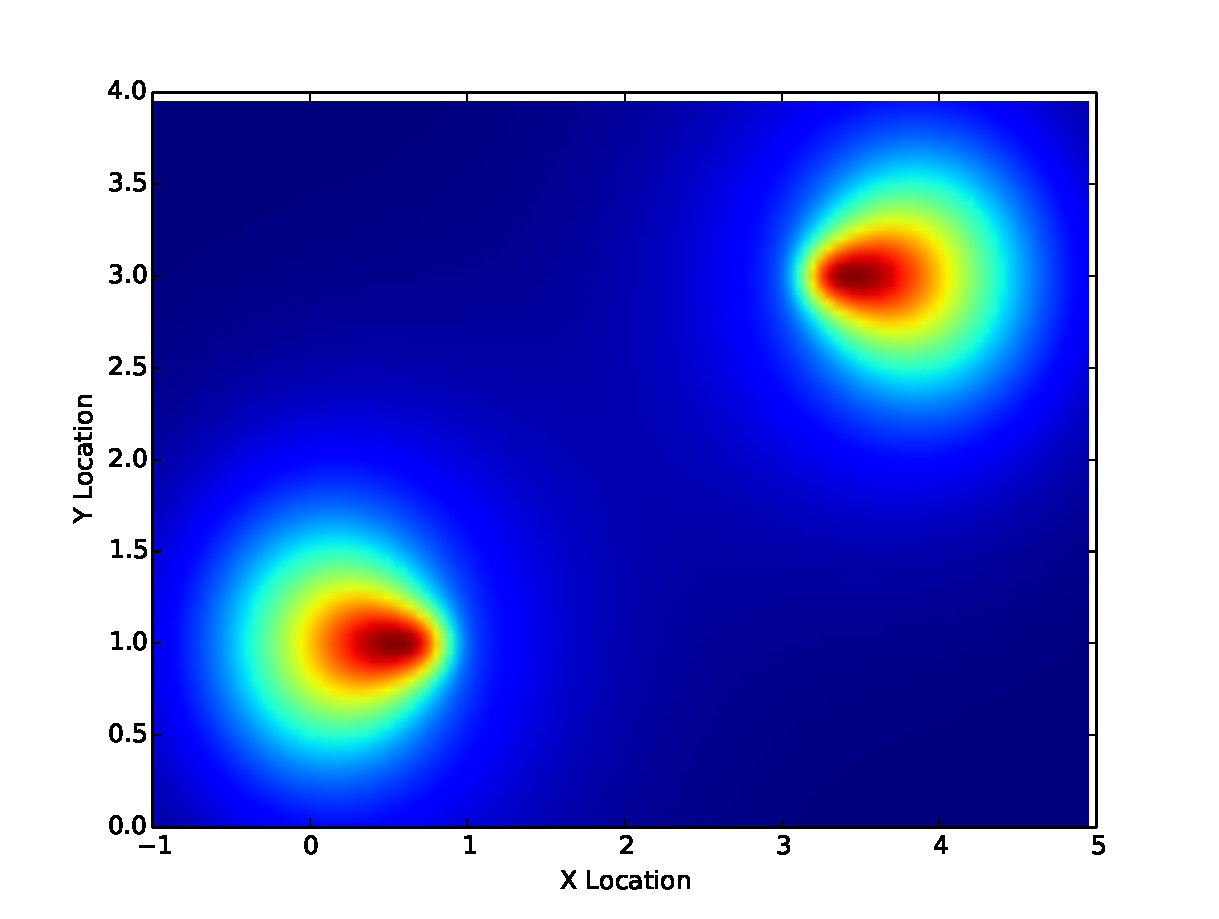
\includegraphics[width=0.24\linewidth]{figs/agent_7}
    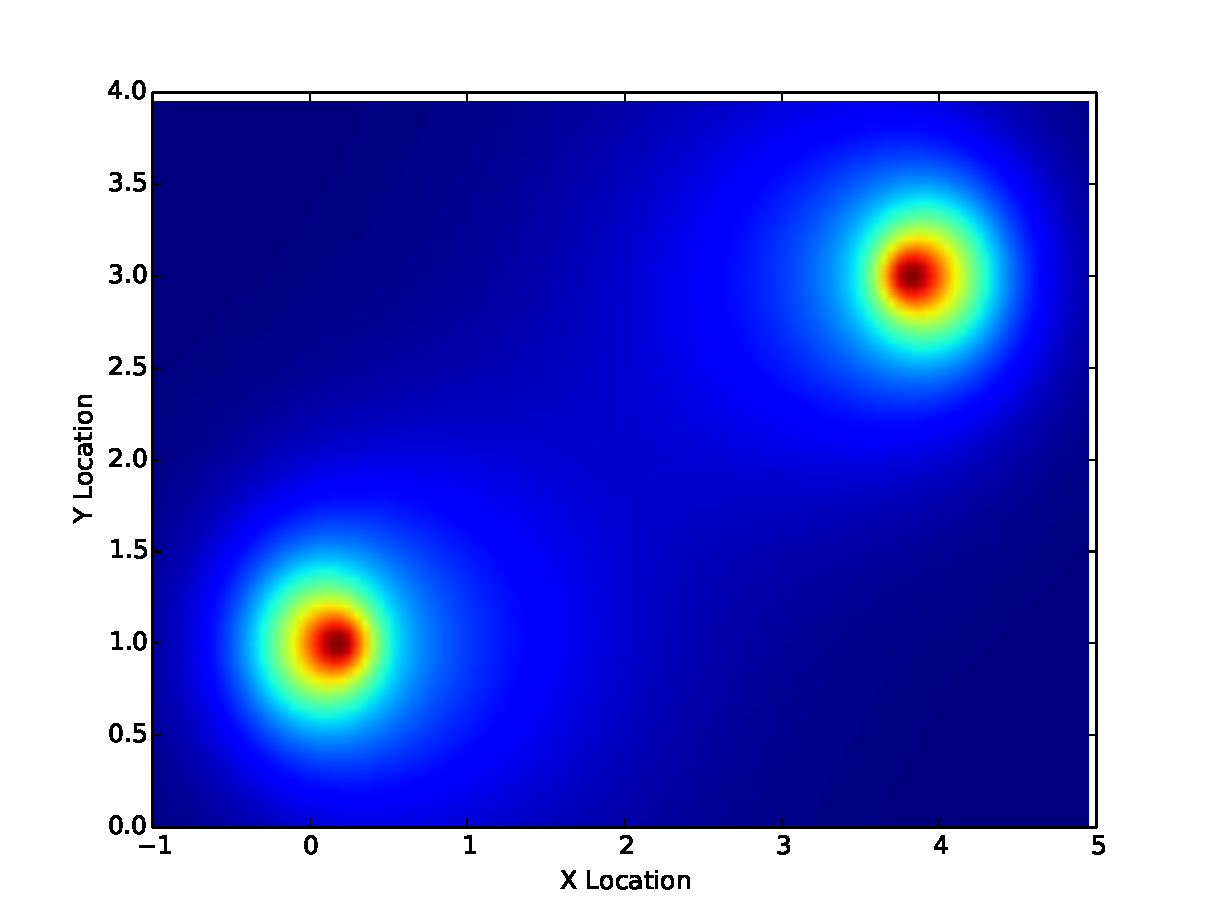
\includegraphics[width=0.24\linewidth]{figs/agent_8}

    \caption{Cost distributions indicating the likelihood that an agent will be
    at a certain location within a given time interval.  These figures show how
this distribution changes over time (left to right, top to bottom)}

    \label{fig:agent_cost}

\end{figure}

\section{Planning Algorithm}

% Graph cost function

\begin{equation}
    C_A(i, j) = \int^1_0 \exp{\Big(
        P_A(x(\lambda), y(\lambda), i_t, j_t) + 1 \Big)
    } \cdot ||i - j||_{2} \,\mathrm{d}\lambda
    \label{eq:cost}
\end{equation}

Where $x(\lambda) = (j_x - i_x) \cdot \lambda + i_x$ and $y(\lambda) = (j_y -
i_y) \cdot \lambda + i_y$ are the parametric equations of the line from $i$ to
$j$.


% Algorithm to generate a roadmap
\begin{algorithm}[ht]
    \caption{$\Function{Roadmap}(n, d, w, h, O)$}
    \algorithmicrequire{
        \\$n$: Maximum number of samples
        \\$d$: Maximum distance between neighbouring nodes
        \\$O$: Set of obstacles
    }
    \\\algorithmicensure{
        \\An unweighted graph of points describing the
        connectivity of the environment
    }
    \label{algo:prm}
    \begin{algorithmic}[1]
        \setcounter{ALC@line}{0}
        \vspace*{1mm}

        \FOR{$i = 1$ \TO $n$}
            \STATE $q \leftarrow \Function{RandomPoint2D}(w, h)$
            \IF{$\bigwedge_{o \in O} \neg \Function{Collision}(o, q)$}
                \STATE $V \leftarrow V \cup \{q\}$
            \ENDIF
        \ENDFOR

        \FORALL{$q_i \in V$}
            \FORALL{$q_j \in V$}
                \IF{$q_i \neq q_j \wedge ||q_i - q_j|| \leq d$}
                    \STATE $E \leftarrow E \cup \{(q_i, q_j)\}$
                    % \STATE $E \leftarrow E \cup \{(q_j, q_i)\}$
                \ENDIF
            \ENDFOR
        \ENDFOR
        \RETURN $(V,E)$
    \end{algorithmic}
\end{algorithm}

% Main algorithm to get the path
\begin{algorithm}[ht]
    \caption{$\Function{GetPath}(n, d, w, h, \delta, p, g, O, A, R)$}
    \algorithmicrequire{
        \\$n$: Maximum number of samples for the roadmap
        \\$d$: Maximum distance between neighbouring nodes in the roadmap
        \\$w$: Width of the scene
        \\$h$: Height of the scene
    }
    \\\algorithmicensure{}
    \label{algo:path}
    \begin{algorithmic}[1]
        \setcounter{ALC@line}{0}
        \STATE $(V, E) \leftarrow \Function{Roadmap}(n, d, w, h, O)$
        \STATE $\Pi \leftarrow \emptyset$
        \STATE $q \leftarrow p$
        \WHILE {$||\Function{Back}(\Pi) - g||_2 > R$}
            \STATE $\pi \leftarrow \Function{SearchGraph}(V, E, R, A, q, g)$
            \FORALL {$i \in \pi$}
                \STATE $\Pi \leftarrow \Pi \cup \{i\}$
                \FORALL {$a \in A$}
                    \STATE $\Function{Step}(a)$
                \ENDFOR
                \IF {$\bigvee_{a \in A} ||\tilde{\zeta_a}(i_t) -
                    \zeta_a(i_t)|| > \delta$}
                    \FORALL {$a \in A$}
                        \STATE $\Function{Update}(\zeta_a, \tilde{\zeta_a})$
                    \ENDFOR
                    \STATE $q \leftarrow i$
                    \STATE $\textbf{break}$
                \ENDIF
            \ENDFOR
        \ENDWHILE
        \RETURN $\Pi$
    \end{algorithmic}
\end{algorithm}

% Algorithm to search the graph
\begin{algorithm}[ht]
    \caption{$\Function{SearchGraph}(V, E, R, A, p, g)$}
    % \algorithmicrequire{}
    % \\\algorithmicensure{}
    \label{algo:search}
    \begin{algorithmic}[1]
        \setcounter{ALC@line}{0}
        \vspace*{1mm}
        \STATE $Q \leftarrow \Function{PriorityQueue}()$
        \STATE $D \leftarrow \Function{Dictionary}()$
        \STATE $\Pi \leftarrow \Function{Dictionary}()$
        \STATE $\Function{Insert}(Q, p, 0)$
        \WHILE {$\neg \Function{Empty}(Q)$}
            \STATE $q, w \leftarrow \Function{Pop}(Q)$
            \IF{$||q - g||_2 \leq R$}
                \RETURN $\Function{BacktrackPath}(p, g, \Pi)$
            \ENDIF
            \STATE $N \leftarrow \Function{GetTemporalNeighbours}(V, E, q)$
            \FORALL{$n \in N$}
                \STATE $\Pi_n \leftarrow q$
                \STATE $c \leftarrow \psi \cdot C_A(q, n) + \omega \cdot D_n$
                \STATE $D_n \leftarrow D_n + 1$
                \STATE $Q \leftarrow \Function{Insert}(Q, n, c)$
            \ENDFOR
        \ENDWHILE
    \end{algorithmic}
\end{algorithm}

% Gets the neighbours in space-time
\begin{algorithm}[ht]
    \caption{$\Function{GetTemporalNeighbours}(V, E, q)$}
    % \algorithmicrequire{}
    % \\\algorithmicensure{}
    \label{algo:neighbours}
    \begin{algorithmic}[1]
        \setcounter{ALC@line}{0}
        \vspace*{1mm}
        \STATE $S \leftarrow \emptyset$
        \STATE $N \leftarrow \Function{Neighbours}(V, E, q)$
        \FORALL {$n \in N$}
            \STATE $t \leftarrow ||q - n||_2 / s + q_t$
            \STATE $S \leftarrow S \cup \{(n_x, n_y, t)\}$
        \ENDFOR
    \end{algorithmic}
\end{algorithm}

% Given a parent dictionary, this returns the backtracked path
\begin{algorithm}[ht]
    \caption{$\Function{BacktrackPath}(p, g, \Pi)$}
    % \algorithmicrequire{}
    % \\\algorithmicensure{}
    \label{algo:backtrack}
    \begin{algorithmic}[1]
        \setcounter{ALC@line}{0}
        \vspace*{1mm}
        \STATE $q \leftarrow g$
        \STATE $S \leftarrow \Function{Stack}()$
        \WHILE {$\Pi_q \neq p$}
            \STATE $S \leftarrow \Function{Push}(S, q)$
            \STATE $q \leftarrow \Pi_q$
        \ENDWHILE
        \STATE $S \leftarrow \Function{Push}(S, p)$
        \RETURN $S$
    \end{algorithmic}
\end{algorithm}

\end{document}
